\documentclass[12pt]{article}  % [12pt] option for the benefit of aging markers
\usepackage{amssymb,amsthm}    % amssymb package contains more mathematical symbols
\usepackage{graphicx}          % graphicx package enables you to paste in graphics
\usepackage[document]{ragged2e} 
\usepackage{float}
\usepackage{tabularx}

%%%%%%%%%%%%%%%%%%%%%%%%%%%%%%%%%
%
%    Page size commands.  Don't worry about these
%
\setlength{\textheight}{220mm}
\setlength{\topmargin}{-10mm}
\setlength{\textwidth}{150mm}
\setlength{\oddsidemargin}{0mm}

%%%%%%%%%%%%%%%%%%%%%%%%%%%%%%%%%%%%%%%%%%%%%%%%%%%%%%%%%%%%%%%
%
%    Definitions of environments for theorems etc.
%
\newtheorem{theorem}{Theorem}[section]          % Theorems numbered within sections - eg Theorem 2.1 in Section 2.
\newtheorem{corollary}[theorem]{Corollary}      % Corollaries etc. will be counted as Theorems for numbering
\newtheorem{lemma}[theorem]{Lemma}              % eg Lemma 3.1, ... Theorem 3.2, ... Corollary 3.3.
\newtheorem{proposition}[theorem]{Proposition}
\newtheorem{conjecture}[theorem]{Conjecture}

\theoremstyle{definition}
\newtheorem{definition}[theorem]{Definition}

\theoremstyle{remark}
\newtheorem{remark}[theorem]{Remark}
\newtheorem{example}[theorem]{Example} 
\graphicspath{ {./Images/} }

%%%%%%%%%%%%%%%%%%%%%%%%%%%%%%%%%%%%%%%%%%%%%%%
%
%        Preamble material specific to your essay
%
\title{Logic-Based Solutions to Puzzles and Riddles\\
Deliverable 1: Research Report}
\author{Kyle Dick\\
F20PA Project\\
supervised by
Kathrin Stark}

\begin{document}
\maketitle

\newpage                     % optional page break
\begin{abstract}
Describe the problem that is to be approached.


\end{abstract}

\newpage                     % optional page break
\tableofcontents

\newpage                     % optional page break
\section{Introduction}\label{s:intro}
%
%In recent times a global interest has developed around the linguistic game Wordle. The concept of this puzzle is simple, the user is to guess a five letter word in as few guesses as possible within six attempts. After each guess the computer will inform the user if a letter was in the correct position, denoted as a green highlight, or is contained within the word but not in the correct %position, denoted with a yellow highlight.
The main focus of this project is to investigate solutions to the puzzle game known as Mastermind. The approach will be to develop an initial base solution in a functional programming language which can be iteratively improved with the goal of creating a solution which is logically sound and efficient.
Mastermind is a simple code-breaking game in which one player will create a secret code which conists of four coloured pegs from a choice of six. This is the standard version of the game however there are multiple variations of the game, some of which will be discussed and examined within the scope of this project.

\subsection {Aims and Objectives}
\begin {itemize}

\item{Aim 1: To derive a solution to Mastermind using logic and equational reasoning.}
	\begin {itemize}
	\item{Objective 1A: Investigate solutions to similar problems. This will give an idea of how an implementation should be approached.}
	\item{Objective 1B:  Implement a base solution using simple logic without consideration to efficiency. This basic solution should only be concerned with giving a foundation that can be 		refined in later iterations.}
	\item{Objective 1C: Iterate and improve on solutions using a declared evaluation process.}
	\end {itemize}
Aim 2: Evaluate solutions and identify a desired solution.
	\begin {itemize}
	\item{Objective 2A: Create an evaluation strategy by identifying which aspects of the solution would best show improvement between iterations.}
	\item{Objective 2B: Analyse an iteration using the chosen strategy.}
	\item{Objective 2C: Report the results of the evaluation strategy and iterate if improvements are identified.}
	\item{Objective 2D: Document results taken to arrive at a desired solution.}
	\end {itemize}
\end {itemize}


%
% The \label command is optional, but useful.  To cross-refer to a section/theorem/equation etc.
% labelled by \label{key}, use \ref{key}.  For example: Equation (\ref{eq:key}) follows from Theorem \ref{th:key}.

\newpage                     % optional page break
\section{Background}\label{ss:back}
This section will provide background material which aims to give context to the aims and objectives of this project. What follows this brief introduction is an explanation of the game Mastermind which the solution will be derived from along with references to previous work by others. The previous work will relate to the field of functional programming and the specific area of logic and equational reasoning. At the conclusion of this section the goal is that the reader has an understanding of the important concepts relating to this project such that the aims and objectives are clear in their feasability and relevancy.

\subsection {Mastermind}
% A brief history and explanation of the game
Mastermind is a code-breaking board game designed by Mordecai Meirowitz originally manufactured by Invicta Toys and Games \cite{Invicta}. 
The original board game consisted of two players with different roles. Player A would be designated the code-breaker while Player B would attempt to solve the code.

The process of the game is as follows.
Player A would first contruct the code from a set of six coloured pegs with the code being exactly four pegs in length. There are variants where the size of the set of choices and code length are variable however this describes the standard variant.

A variant of the original mastermind puzzle was explored 

\begin{figure}[H]
\centering
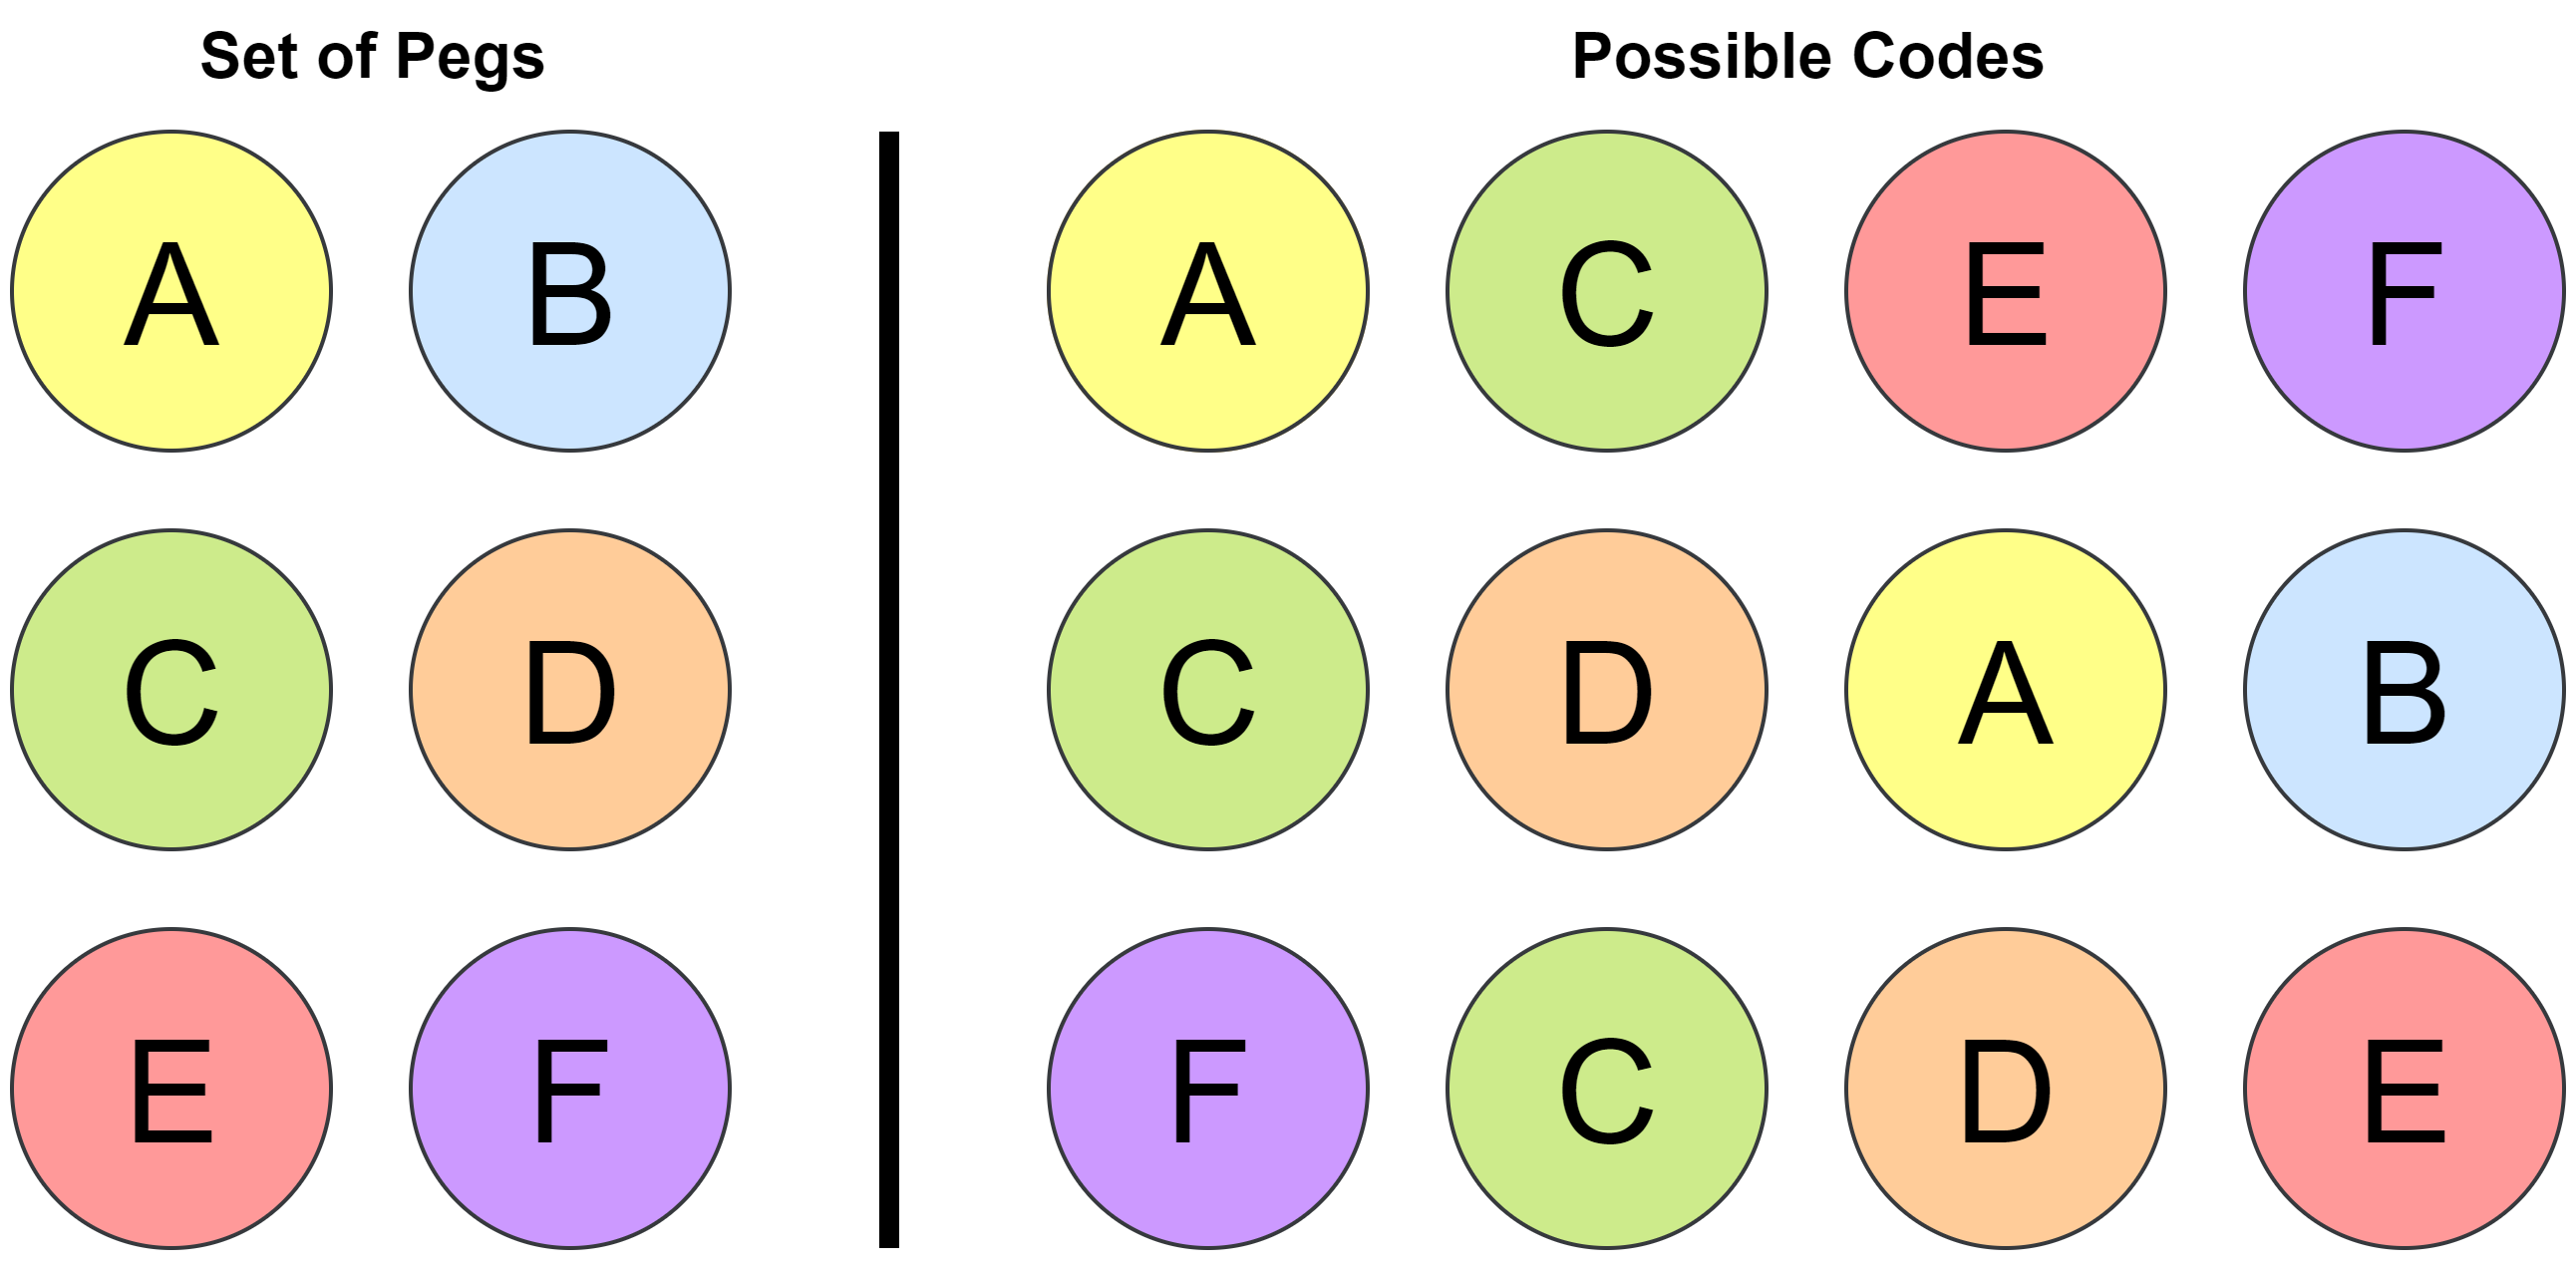
\includegraphics[scale=0.75]{pegs}
\caption{ Example of code enumerations Player A could construct}
\end{figure}

The challenge for Player B is to correctly guess the code created by considering feedback given from Player A relating to how correct each guess was.
A guess is evaluated with Player B given a number of pegs with two possible colours, one which represents a correct position and another which represents a correct colour.

\begin{figure}[H]
\centering
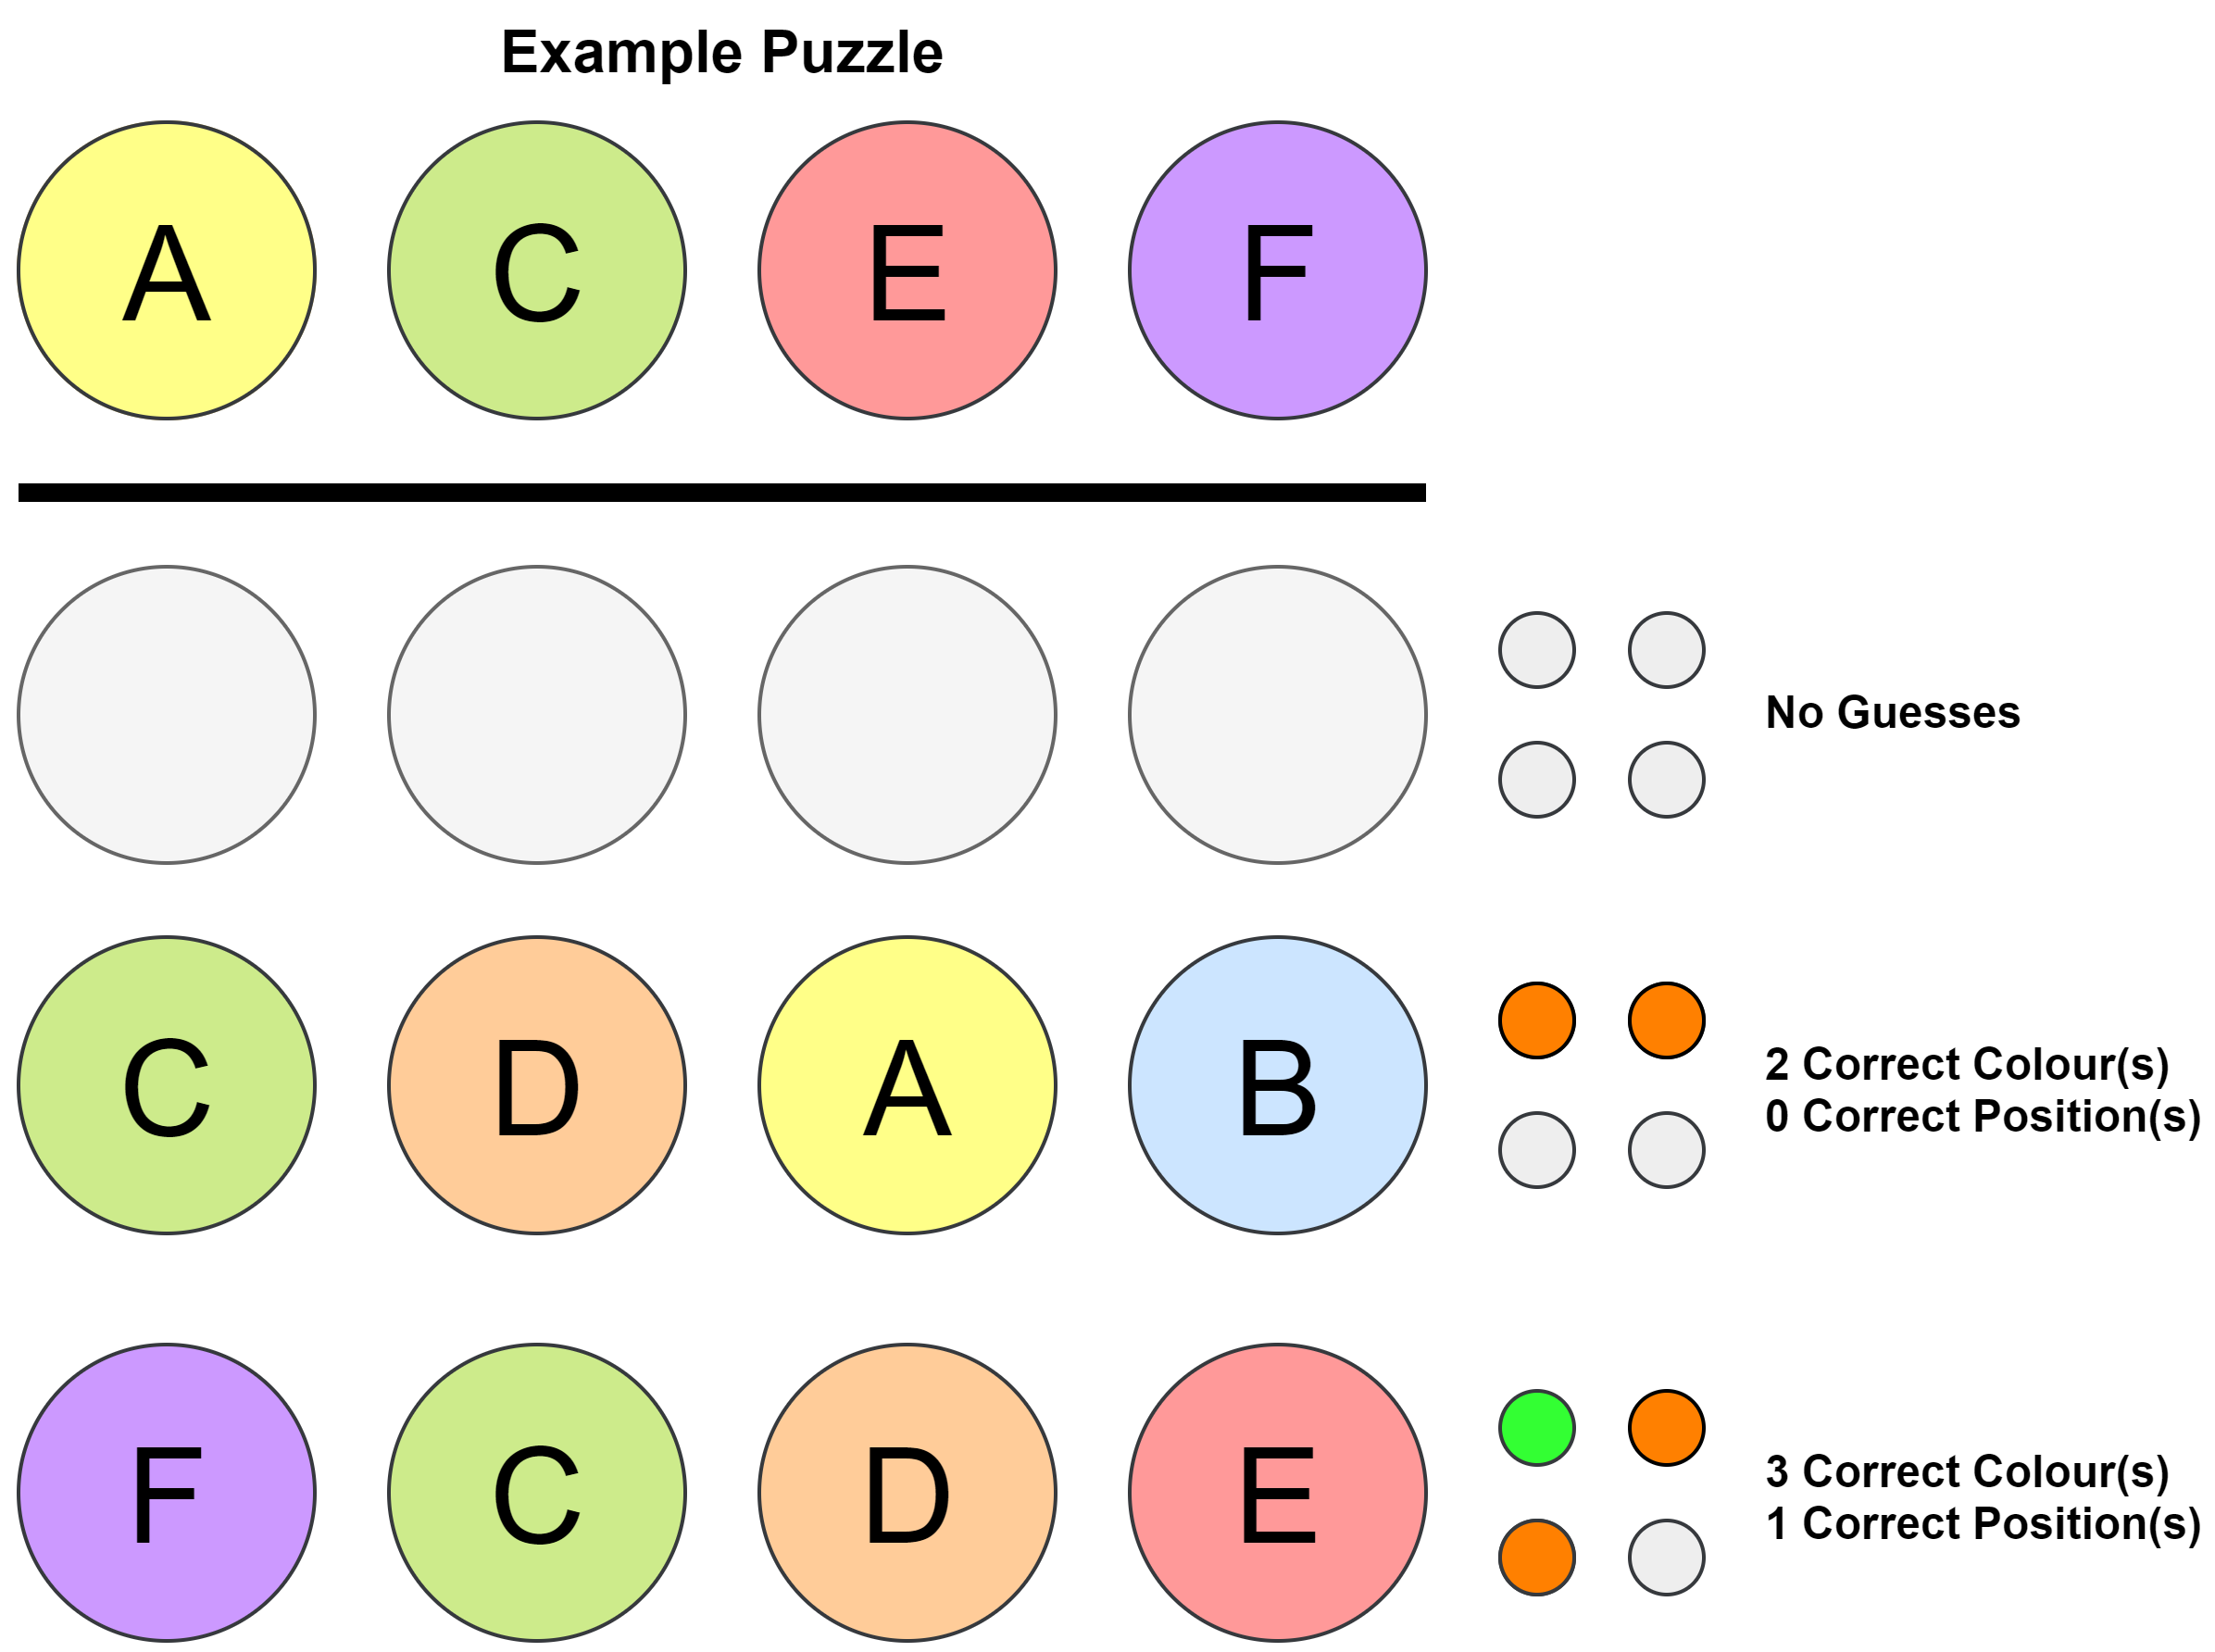
\includegraphics[scale=0.75]{guesses}
\caption{ Simplified example of Player B guesses}
\end{figure}

% A reiteration of the goals with this context
\par The solution that this project aims to implement would assume the role of Player B attempting to correctly identify the generated code in the minimum number of guesses.
To provide a solution which is not bound by the number of elements within the set of possible choices or the length of the code, the code will follow the following rules.

\[ code = [c_i, ... ,c_n]\]
\[pegs = \{c_i, ... , c_m\}\]
\[ n,m = \mathbb{N} > 1\]

% Possible small note about variations and how these could change the goals
A solution which is agnostic of the code length and number of possible elements would support basic variants of Mastermind where the only difference are these restrictions. The base solution will solely focus on solving for a code of length four with six possible elements.

[This section should be extended with discussion of Clear Mastermind with focus paid to the foundation laid out by the researchers involved.

\subsection {Functional Pearls}
% What are Functional Pearls and why introduce the concept
The solution that this project seeks to implement will utilise functional programming to acheive its goals. This required an analysis of similar problems which have seen investigation in the field. An area which proves useful for this area of research is the topic of Functional Pearls.

Functional Pearls are examples of programming which aim to teach important programming techniques and fundamental design principles \cite{Pearls}. Functional Pearls focus on brief but engaging examples that showcase either a guided explanation to a program calculation or proof or presenation of unique data structures. The encompassing feature of Functional Pearls is that they showcase educational material in a way that is digestable and entertaining.

% Are there any that would be relevant to this (Simple Sudoku Solver)
A functional Pearl example which holds relevance to the current project is Richard Bird's 'A Program to Solve Sudoku' \cite{Sudoku}. This paper focused on using equational reasoning over mathematics to implement a solution to sudoku puzzles written in Haskell. This solution is relevant to the current project due to the factor they share similar problems of code breaking. The approach of this solution was to start with a base solution which would generate a large volume of possible boards which would be matched to a given input. The conclusion of the study resulted in an elegant solution which would apply equational reasoning to derive a function capable of giving multiple possible solutions to the given input. The limitations were compared to similar solutions which showed a struggle with larger inputs but an increase over other implementations with simplified board states.


\subsection {Logic and Equational Reasoning}
% Discussion of what a logical approach to programming would be
The goal with the solution this project aims for is to implement a solution which is logically sound. This means for the project to succeed

% Equational Reasoning vs Maths

\newpage                     % optional page break
\section{Research Methodology}\label{ss:back}

\newpage                     % optional page break
\section{Evaluation Strategy}\label{ss:back}


\newpage                     % optional page break
\section{Project Management}\label{ss:back}

\subsection {File and Resource Management}

\subsection {Timeline and Deadlines}

\subsection {Risk Analysis and Mitigations}

To manage the progress of this project efficiently it was important to identify possible risks that could prevent the realisation of the goals laid out earlier in this document. To aid in the identification of the risks the following key was used to classify the associated risks:
\begin{itemize}
\item{People (P) - Risks which are the result of issues related to those individuals involved in the engineering of solutions.}
\item{Technological (T) - Risks which result from the technology being used to engineer the solutions. This involves the software, hardware and frameworks used.}
\item{Requirement (R)  - Risks which result from changes to the requirements of the project. Examples of such being a requirement being dropped from the scope or a requirements priority undergoing a change.}
\item{Estimation (E) - Risks which result from ill estimations of the project timing, capabilities of an individual or understanding of a certain technology.}
\end{itemize}

\begin{tabularx}{1.1\textwidth} {
	|  >{\center\arraybackslash}X
	| >{\center\arraybackslash}X
	| >{\center\arraybackslash}X
	| >{\center\arraybackslash} X | }
	\hline
	ID & Risk & Risk Type & Description \\
	\hline
	P/T/R/E1 & Textual Title of Risk & Class of Risk & Textual Description of the Risk \\
	\hline
\end{tabularx}



%%%%%%%%%%%%%%%%%%%%%%%%%%%%%%%%%%%%%%%%%
%
%     Bibliography
%
%     Use an easy-to-remember tag for each entry - eg \bibitem{How97} for an article/book by Howie in 1997
%     To cite this publication in your text, write \cite{How97}.  To include more details such as
%     page, Chapter, Theorem numbers, use the form \cite[Theorem 6.3, page 42]{How97}.
%
\begin{thebibliography}{99}

% 
% The usual convention for mathematical bibliographies is to list alphabetically
% by first-named author (then second, third  etc. author then date)
% websites with no author names should go by the site name
%

% Typical layout for reference to a journal article
%\bibitem{Bovey}
%J. D. Bovey, M. M. Dodson,                         % author(s)
%The Hausdorff dimension of systems of linear forms % article name
%{\em Acta Arithmetica}                             % journal name - italics
%{\bf 45}                                           % volume number - bold
%(1986), 337--358.                                   % (year), page range


% Typical layout for reference to a book
%
%\bibitem{Cassels}
%J. W. S. Cassels,                                  % author(s)
%{\em An Introduction to Diophantine Approximation},% title - italics
%Cambridge University Press, Cambridge, 1965.       % Publisher, place, date.

% Typical layout for reference to a website
%
%\bibitem{GAP}
%The GAP Group, GAP -- Groups, Algorithms, and Programming,  % Site name
%Version 4.5.6; 2012. % other information
%(http://www.gap-system.org)  % URL


% Typical layout for reference to an online article

%\bibitem{Howie}
%J. Howie,                                            % author(s)
%{\em Generalised triangle groups of type $(3,5,2)$}, % article name - italics
%http://arxiv.org/abs/1102.2073                       % URL
%(2011).                                              % (year)

\bibitem {Invicta}
Invicta Toys and Games ltd,
{\em History of Mastermind}
https://web.archive.org/web/20070812104420/http://dspace.dial.pipex.com/town/road/gbd76/toys.htm
(Archived 2007)

\bibitem {Pearls}
Jeremy Gibbons,
{\em University of Oxford, Functional Pearls}
http://www.cs.ox.ac.uk/people/jeremy.gibbons/pearls/
(2009)

\bibitem {Sudoku}
Richard Bird
{\em Functional Pearl, A Program to Solve Sudoku}
Cambridge University Press, Cambridge, 2006

\end{thebibliography}
\end{document}
